%-----------------------
% Title page
%-----------------------
\begin{titlepage}
  \centering

  \textsc{ELEC4630 Assignment 2}\\
  \vspace{9cm}

  \rule{\linewidth}{0.5pt}\\

  \vspace{1em}
  \LARGE\textsc{Question 2}\\
  \vspace{1em}

  \LARGE\uppercase{\textbf{{3D Reconstruction}}}\\

  \rule{\linewidth}{2pt}\\

  \vfill

  \normalsize{Deren Teo (4528554)}
  \vspace{1cm}

\end{titlepage}

%-----------------------
% Report body
%-----------------------
\section{Introduction}

Dense 3D reconstruction from multiple RGB images has long been a topic of interest in computer vision, and serves numerous practical purposes \cite{ulusoy_2016}. For example, 3D reconstruction applied to medical imaging can enable medical experts to better visualise areas of interest, for more accurate dianoses and better planning of medical procedures \cite{icoi_nd}. 3D reconstruction also has applications in a civil engineering context, to reconstruct models of buildings, roads, bridges, and other structures from 3D point clouds \cite{ma_2018}.

One well-established technique for 3D reconstruction is shape-from-silhouette (SHS) \cite{cheung_2005}. SHS estimates a 3D reconstruction based on silhouettes of an object from multiple view points \cite{cheung_2005}. This report presents one attempt at using SHS to reconstruct the well-known Oxford Dinosaur using the standard data set of 36 images \cite{schoning_2015}.

\newpage
\section{Background Theory}

\subsection{Projective Geometry}

Projective geometry is a branch of mathematics concerned with the transforms associated with projecting geometric shapes onto a surface \cite{artmann_2018}. The concept is of foundational relevance to SHS because a silhouette is the projection of a shape in 3D space onto a 2D surface.

Consider the illustration of Figure \ref{fig:projective_geometry}, demonstrating the projection of a 3D object.

\begin{figure}[ht]
  \centering
  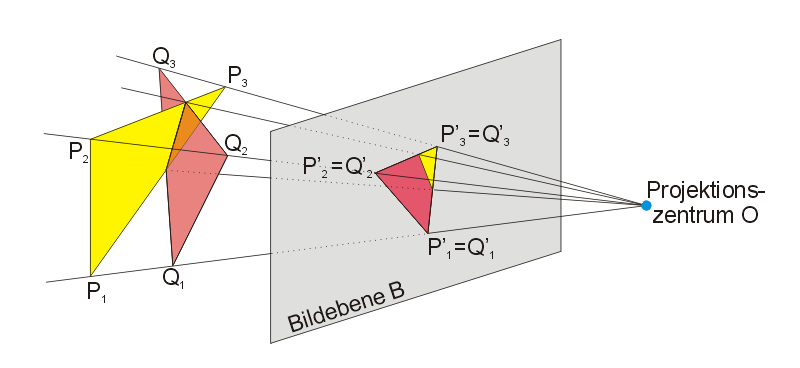
\includegraphics[width=0.6\textwidth]{images/q2_projective_geometry.jpg}
  \caption{Projection of a 3D object onto a 2D surface from a projection centre \cite{baecker_2005}.}
  \label{fig:projective_geometry}
\end{figure}

Intuitively, the projected image depends on the relative orientation of the surface and the object, and also on the distance between the projection centre and both the object and the surface. The orientation determines the projected image, and the distance defines the scale of the projection.

To capture the size of an object in a projection, since this varies with distance to the projection centre, projective geometry includes an additional coordinate, $w$, in addition to the standard Cartesian coordinates $x$ and $y$ (and $z$ in 3D space) \cite{lovell_2023b}. The additional coordinate specifies the distance between the projection and the projection centre \cite{lovell_2023b}.

Converting between projective and Cartesian coordinates in both 2D and 3D is simple \cite{lovell_2023b}:
\begin{align}
  \text{In 2D: } (x, y, w) \longleftrightarrow \left( \frac{x}{w}, \frac{y}{w} \right) &&
  \text{In 3D: } (x, y, z, w) \longleftrightarrow \left( \frac{x}{w}, \frac{y}{w}, \frac{z}{w} \right)
\end{align}

Given the additional coordinate, $w$, if the pose of the projection centre is known, then it is possible to determine the size of the projected object.

Conversely, the projection of an object onto a surface can be calculated using a projective matrix, $P$. For the projection of a 3D object onto a 2D surface, the projective matrix has dimensions $3\times4$ \cite{lovell_2023b}, and internally captures all necessary information regarding the pose of the projection centre relative to the object.

Using projective coordinates, the projection of a point in 3D space relative to a surface and projection centre specified by some projection matrix is realised on the 2D surface as \cite{lovell_2023b}:
\begin{align}
  \begin{bmatrix}
    p_{11} & p_{12} & p_{13} & p_{14} \\
    p_{21} & p_{22} & p_{23} & p_{24} \\
    p_{31} & p_{32} & p_{33} & p_{34} \\
    p_{41} & p_{42} & p_{43} & p_{44} \\
  \end{bmatrix}
  \begin{bmatrix}
    x \\
    y \\
    z \\
    w \\
  \end{bmatrix}
  =
  \begin{bmatrix}
    x_i \\
    y_i \\
    w_i \\
  \end{bmatrix}
\end{align}

In the inverse direction, however, given a projection centre pose, estimating the projection matrix is a non-trivial task \cite{lovell_2023b}. For the purposes of this investigation, projection matrices are known for all projections; therefore, no determination of projection matrices is necessary.

\newpage
\subsection{Shape-From-Silhouette}

Shape-from-silhouette (SHS) is a method of 3D reconstruction using silhouettes of an object as viewed from multiple known positions \cite{lovell_2023b}. In the nomenclature of projective geometry, a silhouette is a 2D projection of an object in 3D space, formed by the intersection of the visual cone of a ``camera'' at the projection centre \cite{cheung_2005}. Using a sufficient number of silhouettes from cameras with different relative poses, the 3D object can be approximately reconstructed as the intersection of the various visual cones \cite{lovell_2023b}. This is demonstrated by Figure \ref{fig:silhouettes}.

\begin{figure}[ht]
  \centering
  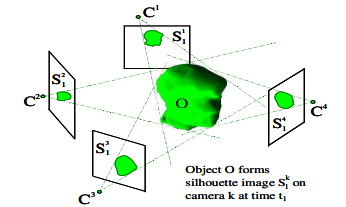
\includegraphics[width=0.5\textwidth]{images/q2_shape_from_silhouette.png}
  \caption{Silhouettes formed by the intersections of visual cones with a surface (from \cite{cheung_2005}).}
  \label{fig:silhouettes}
\end{figure}

The algorithm is programatically simple. The 3D reconstruction begins as a solid bounding box around the object of interest. Given a silhouette and an associated projection matrix, which defines the projective transformation between points in 3D space and points on the silhouette plane, each point in the reconstruction is projected onto the silhouette plane and compared with the silhouette. If the projected point lies outside the silhouette, then it is removed from the reconstruction. This is performed for all points in the reconstruction, and repeated for all available silhouettes. Once the algorithm concludes, the remaining shape is an approximate reconstruction of the original 3D object; the accuracy of the reconstruction depends on the number of silhouettes and the geometry of the object.

For example, Figure \ref{fig:shs_example} presents three SHS reconstructions of the same 3D model using an increasing number of silhouettes. The difference in reconstruction quality is evident.

\begin{figure}[ht]
  \centering
  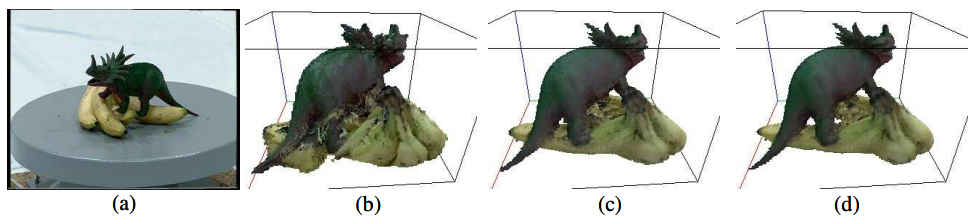
\includegraphics[width=0.8\textwidth]{images/q2_shape_from_silhouette_example.png}
  \caption{Coloured reconstructions of (a) using 6 (b), 36 (c), and 66 (d) silhouettes (from \cite{cheung_2005}).}
  \label{fig:shs_example}
\end{figure}

The advantages of SHS for 3D reconstruction include the easy availability of silhouettes, especially in an indoor environment with static cameras and controlled lighting \cite{cheung_2005}. For example, the Oxford Dinosaur dataset is derived from a single static camera capturing photographs at regular intervals of a dinosaur toy on a turntable. The colour of the photograph backgrounds makes it easy to segment a silhouette of the dinosaur.

However, SHS also has certain limitations. Foremost among these are that the quality of the reconstruction is highly dependent on the number of distinct silhouettes \cite{cheung_2005}. The method can also be sensitive to noise in segmented silhouettes \cite{lovell_2023b}. Finally, the method always produces a conservative reconstruction, and inherently cannot model convexities \cite{cheung_2005}.

\newpage
\section{Methodology}

\section{Results}

\section{Discussion}

\section{Conclusion}